%-------------------------------------------------------------------------------------------------------
%
%
%-------------------------------------------------------------------------------------------------------
\documentclass[a4paper,11pt]{book} 

%-------------------------------------------------------------------------------------------------------
% Get all packages and styles.
%
%-------------------------------------------------------------------------------------------------------
%-------------------------------------------------------------------------------------------------------
% Packages
%
%-------------------------------------------------------------------------------------------------------
\usepackage{amsmath}           
\usepackage{hyperref}           
\usepackage{geometry}           
\usepackage{fancyhdr}           
\usepackage{titlesec}
\usepackage{titlepic}
\usepackage{booktabs}
\usepackage{listings}
\usepackage{xcolor}
\usepackage{tcolorbox}
\usepackage{graphicx}           
\usepackage{pdfpages}
\usepackage{float}
\usepackage{placeins}
\usepackage{tikz}
\usepackage{relsize}
\usepackage{pdflscape}
\usepackage{tabularx}
\usepackage{longtable}
\usepackage{array}
\usepackage[all]{nowidow}
\usepackage{etoolbox}
\usepackage{tocloft}
%\usepackage[scaled]{beramono}
\usetikzlibrary{shapes,shadows,arrows,calc,intersections}
\usetikzlibrary{decorations.pathreplacing}

%-------------------------------------------------------------------------------------------------------
%
%
%
%-------------------------------------------------------------------------------------------------------

%-------------------------------------------------------------------------------------------------------
% Page layout settings
%
%-------------------------------------------------------------------------------------------------------
\geometry{a4paper, margin=1in, top=1in, bottom=1in, left=1in, right=1in, headheight=0.5in}
\addtolength{\parskip}{1.0ex}

\pagestyle{fancy}               
\fancyhf{}                     
\fancyhead[L]{\leftmark}       
\fancyfoot[R]{\thepage}         
\renewcommand{\headrulewidth}{0pt}
\renewcommand{\footrulewidth}{0pt}

%-------------------------------------------------------------------------------------------------------
% Force all "plain" pages (chapter starts, TOC, etc.) to use fancy layout
%
%-------------------------------------------------------------------------------------------------------
\makeatletter
\let\ps@plain\ps@fancy
\makeatother


%-------------------------------------------------------------------------------------------------------
% Chapter title settings 
%
%-------------------------------------------------------------------------------------------------------
\titleformat{\chapter}[hang]{\normalfont\huge\bfseries}{\thechapter}{2pc}{}
\titlespacing*{\chapter}{0pt}{0.1in}{0.2in}

%-------------------------------------------------------------------------------------------------------
% Table of Content settings 
%
%-------------------------------------------------------------------------------------------------------
\setlength{\cftsubsecindent}{1cm}
\setlength{\cftsubsubsecindent}{2cm}

%-------------------------------------------------------------------------------------------------------
% Listing style for showing code snippets. This style is used for showing short code sequences.
%
%-------------------------------------------------------------------------------------------------------
\lstdefinestyle{codesnippetstyle}{
    backgroundcolor=\color{gray!5},
    basicstyle={\ttfamily\tiny}, % Try \relsize{-2} if this is still too large
    keywordstyle=\color{magenta},
    identifierstyle={\ttfamily\color{blue}},
    numberstyle={\ttfamily\footnotesize\color{gray}},
    commentstyle={\ttfamily\color{teal}},
    showstringspaces=false,
    numbers=left,
    frame=single,
    texcl=false,
    alsoletter={\#},
    morekeywords={\#include, \#define, \#ifdef, \#endif, \#pragma},
    linewidth=0.9\textwidth,
    xleftmargin=0.1\textwidth,
    breaklines=true,
    breakatwhitespace=false,
    columns=fullflexible
}

%-------------------------------------------------------------------------------------------------------
% Common TIKZ styles for my pictures.
%
%---------------------------------------------------------------------------------------------------
\tikzstyle{tsLargeBold} = [ 
    text=black, 
    font=\bfseries\large
]

\tikzstyle{tsWraptext} = [ 
    tsLargeBold, 
    text centered, 
    align=left
]

\tikzstyle{tsRectangle} = [ 
    rectangle,
    tsWraptext,               
    draw=black,
    line width=0.25mm]

\tikzstyle{tsRoundedRectangle} = [  
    tsRectangle,
    rounded corners
]

\tikzstyle{tsCircle} = [   
        circle,
        tsWraptext,
        draw=black,
        line width=1mm
    ]

\tikzstyle{tsEllipse} = [   
    ellipse,
    tsWraptext,
    draw=black,
    line width=1mm
]

%-------------------------------------------------------------------------------------------------------
% Instruction format pages use this layout.
%
%-------------------------------------------------------------------------------------------------------
\newcommand{\instructionentry}[2]{%
  \noindent
  \begin{minipage}[t]{0.22\textwidth}
    \textbf{\large\textcolor{blue}{#1}}%
  \end{minipage}%
  \hfill
  \begin{minipage}[t]{0.74\textwidth}
    #2
  \end{minipage}\par\vspace{0.75em}
}



%-------------------------------------------------------------------------------------------------------
% Document start.
%
%-------------------------------------------------------------------------------------------------------
\begin{document}
	
	%---------------------------------------------------------------------------------------------------
    % Options to deal with how a line is filled.
    %
    %---------------------------------------------------------------------------------------------------
    \setlength{\emergencystretch}{3em}
    \raggedbottom
     
    %---------------------------------------------------------------------------------------------------
    % Title page.
    %
    %---------------------------------------------------------------------------------------------------
    \begingroup
  		\let\cleardoublepage\relax
  		\pagestyle{empty}
  		\pagenumbering{gobble}
  		\begin{titlepage}
    		\begin{center}
    		    			
      			{\Huge \textbf{TWIN-64}} \\
      			{\LARGE \textbf{Architecture Document}} 

      			\vspace{2cm}

      			{\LARGE Helmut Fieres} \\
      			{\large \today}
    		\end{center}
  		\end{titlepage}
	\endgroup
		
    %---------------------------------------------------------------------------------------------------
    % Book body.
    %
    %---------------------------------------------------------------------------------------------------
   	\frontmatter 
    \pagestyle{fancy}      
	\tableofcontents   
	\markboth{ } { }
		
	\mainmatter   
    \pagestyle{fancy}
    
    \chapter*{Introduction}
\addcontentsline{toc}{chapter}{Introduction}


\section*{Instruction Formats}
\addcontentsline{toc}{section}{Instruction Formats}

\begin{center}
    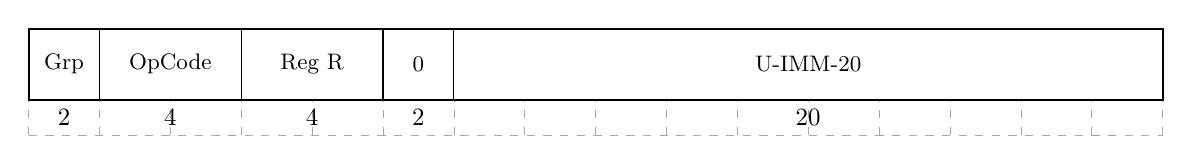
\begin{tikzpicture}[scale=0.9, transform shape]
        
        \draw[help lines, gray!70, dashed] (0,0) grid(16,1.5);
        
        \node[  tsRectangle, 
                minimum width=16cm,
                minimum height=1cm,
                text width=3cm,
                text centered,
                fill=white!50] (blocks) at (8,1) { };
                
     	\draw[-] (1,0.5) -- (1,1.5);
     	\draw[-] (3,0.5) -- (3,1.5);
     	\draw[-] (5,0.5) -- (5,1.5);
     	\draw[-] (6,0.5) -- (6,1.5);
     	     	
     	\node at (0.5,0.25) {2};
    	\node at (2,0.25) {4};
    	\node at (4,0.25) {4};
    	\node at (5.5,0.25) {2};
   	 	\node at (11,0.25) {20};
   	 	
   	 	\node at (0.5,1) {\small Grp};
		\node at (2,1) {\small OpCode};
		\node at (4,1) {\small Reg R};
		\node at (5.5,1) {\small 0};
		\node at (11,1) {\small U-IMM-20};
   	 	
       \end{tikzpicture}
\end{center}

\begin{center}
    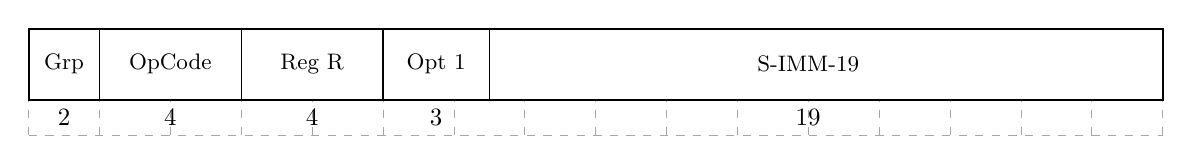
\begin{tikzpicture}[scale=0.9, transform shape]
        
        \draw[help lines, gray!70, dashed] (0,0) grid(16,1.5);
        
        \node[  tsRectangle, 
                minimum width=16cm,
                minimum height=1cm,
                text width=3cm,
                text centered,
                fill=white!50] (blocks) at (8,1) { };
                
     	\draw[-] (1,0.5) -- (1,1.5);
     	\draw[-] (3,0.5) -- (3,1.5);
     	\draw[-] (5,0.5) -- (5,1.5);
     	\draw[-] (6.5,0.5) -- (6.5,1.5);
     	
     	\node at (0.5,0.25) {2};
    	\node at (2,0.25) {4};
    	\node at (4,0.25) {4};
    	\node at (5.75,0.25) {3};
   	 	\node at (11,0.25) {19};
   	 	
   	 	\node at (0.5,1) {\small Grp};
		\node at (2,1) {\small OpCode};
		\node at (4,1) {\small Reg R};
		\node at (5.75,1) {\small Opt 1};
		\node at (11,1) {\small S-IMM-19};
   	 	
       \end{tikzpicture}
\end{center}

\begin{center}
    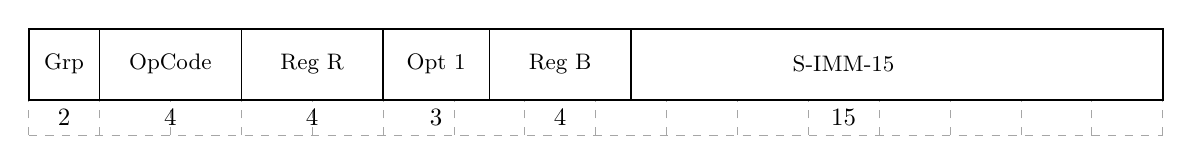
\begin{tikzpicture}[scale=0.9, transform shape]
        
        \draw[help lines, gray!70, dashed] (0,0) grid(16,1.5);
        
        \node[  tsRectangle, 
                minimum width=16cm,
                minimum height=1cm,
                text width=3cm,
                text centered,
                fill=white!50] (blocks) at (8,1) { };
                
     	\draw[-] (1,0.5) -- (1, 1.5);
     	\draw[-] (3,0.5) -- (3, 1.5);
     	\draw[-] (5,0.5) -- (5, 1.5);
     	\draw[-] (6.5,0.5) -- (6.5, 1.5);
     	\draw[-] (8.5,0.5) -- (8.5, 1.5);
          	
     	\node at (0.5,0.25) {2};
    	\node at (2,0.25) {4};
    	\node at (4,0.25) {4};
    	\node at (5.75,0.25) {3};
    	\node at (7.5,0.25) {4};
   	 	\node at (11.5,0.25) {15};
   	 	
   	 	\node at (0.5,1) {\small Grp};
		\node at (2,1) {\small OpCode};
		\node at (4,1) {\small Reg R};
		\node at (5.75,1) {\small Opt 1};
		\node at (7.5,1) {\small Reg B};
		\node at (11.5,1) {\small S-IMM-15};
   	 	
       \end{tikzpicture}
\end{center}

\begin{center}
    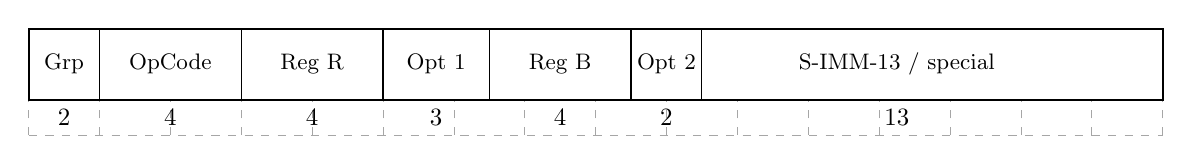
\begin{tikzpicture}[scale=0.9, transform shape]
        
        \draw[help lines, gray!70, dashed] (0,0) grid(16,1.5);
        
        \node[  tsRectangle, 
                minimum width=16cm,
                minimum height=1cm,
                text width=3cm,
                text centered,
                fill=white!50] (blocks) at (8,1) { };
                
     	\draw[-] (1,0.5) -- (1, 1.5);
     	\draw[-] (3,0.5) -- (3, 1.5);
     	\draw[-] (5,0.5) -- (5, 1.5);
     	\draw[-] (6.5,0.5) -- (6.5, 1.5);
     	\draw[-] (8.5,0.5) -- (8.5, 1.5);
     	\draw[-] (9.5,0.5) -- (9.5, 1.5);
     	
     	\node at (0.5,0.25) {2};
    	\node at (2,0.25) {4};
    	\node at (4,0.25) {4};
    	\node at (5.75,0.25) {3};
    	\node at (7.5,0.25) {4};
    	\node at (9,0.25) {2};
     	\node at (12.25,0.25) {13};
   	 	
   	 	\node at (0.5,1) {\small Grp};
		\node at (2,1) {\small OpCode};
		\node at (4,1) {\small Reg R};
		\node at (5.75,1) {\small Opt 1};
		\node at (7.5,1) {\small Reg B};
		\node at (9,1) {\small Opt 2};
		\node at (12.25,1) {\small S-IMM-13 / special};
   	 	
       \end{tikzpicture}
\end{center}



\begin{center}
    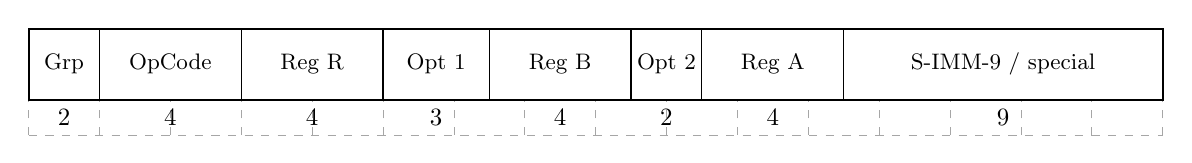
\begin{tikzpicture}[scale=0.9, transform shape]
        
        \draw[help lines, gray!70, dashed] (0,0) grid(16,1.5);
        
        \node[  tsRectangle, 
                minimum width=16cm,
                minimum height=1cm,
                text width=3cm,
                text centered,
                fill=white!50] (blocks) at (8,1) { };
                
     	\draw[-] (1,0.5) -- (1, 1.5);
     	\draw[-] (3,0.5) -- (3, 1.5);
     	\draw[-] (5,0.5) -- (5, 1.5);
     	\draw[-] (6.5,0.5) -- (6.5, 1.5);
     	\draw[-] (8.5,0.5) -- (8.5, 1.5);
     	\draw[-] (9.5,0.5) -- (9.5, 1.5);
     	\draw[-] (11.5,0.5) -- (11.5, 1.5);
     	
     	\node at (0.5,0.25) {2};
    	\node at (2,0.25) {4};
    	\node at (4,0.25) {4};
    	\node at (5.75,0.25) {3};
    	\node at (7.5,0.25) {4};
    	\node at (9,0.25) {2};
    	\node at (10.5,0.25) {4};
   	 	\node at (13.75,0.25) {9};
   	 	
   	 	\node at (0.5,1) {\small Grp};
		\node at (2,1) {\small OpCode};
		\node at (4,1) {\small Reg R};
		\node at (5.75,1) {\small Opt 1};
		\node at (7.5,1) {\small Reg B};
		\node at (9,1) {\small Opt 2};
		\node at (10.5,1) {\small Reg A};
		\node at (13.75,1) {\small S-IMM-9 / special };
   	 	
       \end{tikzpicture}
\end{center}




\section*{This book}


    
    % content goes here ....         
   
    \appendix 
    
    % content goes here ....  

    \backmatter             

\end{document}
